\documentclass[simplex.tex]{subfiles}
% DO NOT INCLUDE PREAMBLES/PACKAGES HERE!!
% packages are inherited from preamble.tex; you can compile this on its own
\begin{document}
\subsection[LOL]{LOL \href{https://github.com/jovo}{@jovo}}

%%% Jan
This quarter we generate simulation results supporting those theoretical claims (see Figure \ref{fig:LOL}).


\begin{figure}[h!]
\begin{cframed}
\centering
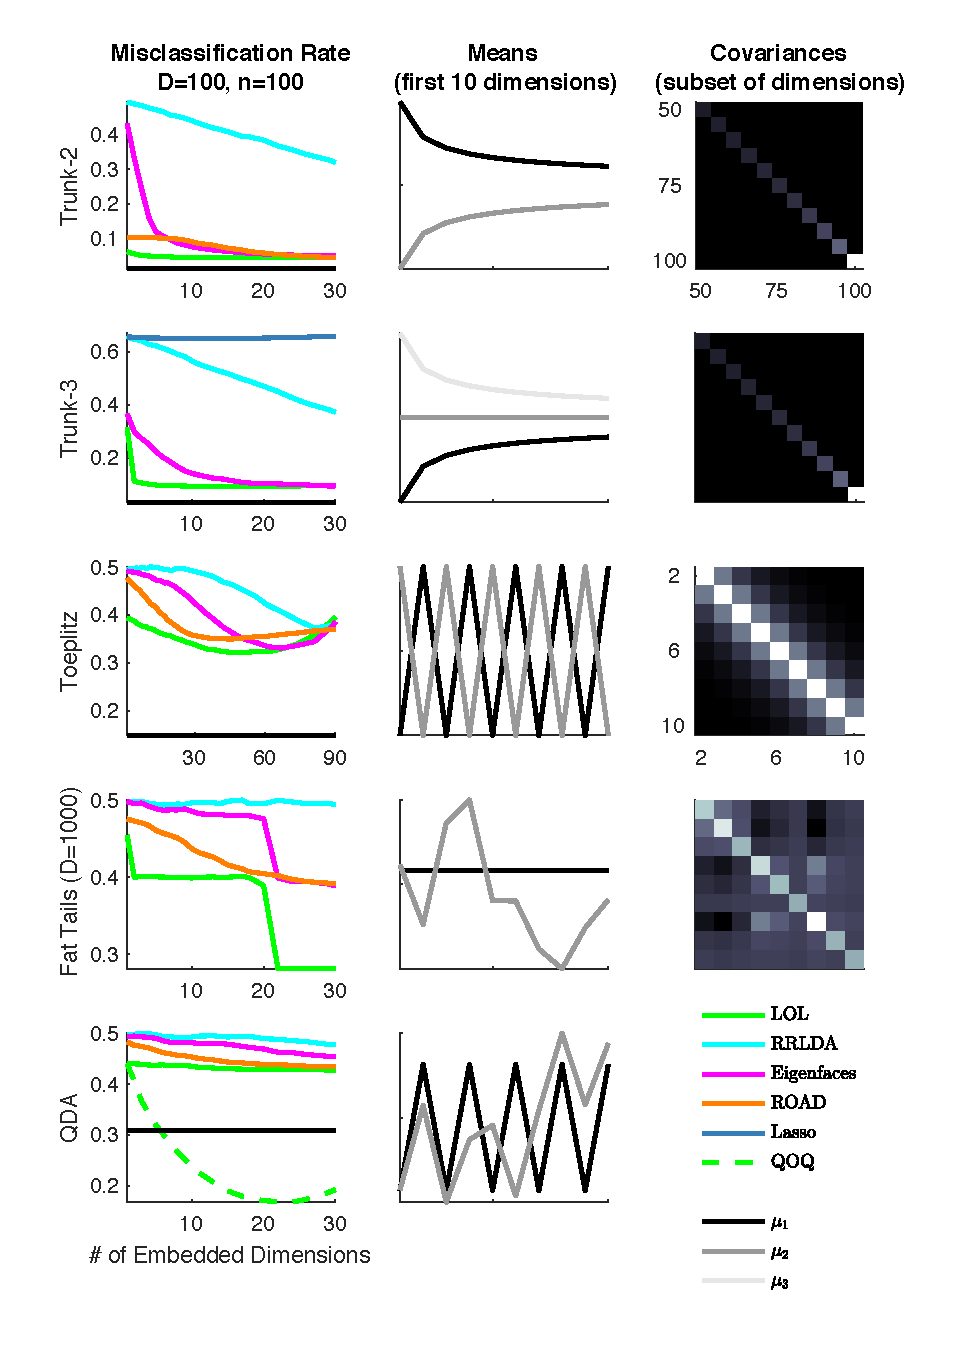
\includegraphics[width=0.7\textwidth]{../../figs/plot_all.pdf}
\caption{
LOL outperforms other linear classifiers in a wide variety of settings, including those for which we have proven LOL should (rows 1 and 3), and those beyond our current theoretical grasp (rows 2, 4, and 5). This is true regardless of the dimensionality into which we embed.
}
\label{fig:LOL}
\end{cframed}
\end{figure}

\clearpage

%%% March
We also finalized the real data analysis using LOL.  In particular, we considered four datasets, the Prostate and Colon datasets have extensively been studied in the sparse literature.  LOL yields better perforance, and for Colon, with lower dimensionality.  MNIST is an even more prominent dataset, LOL achieves the best performance for all dimensions.  MRN is a new dataset that we generated; it has over 500 million features, and 112 samples.  We subsampled to 100 samples for cross-validation purposes.  To our knowledge, no other machine learning tool is capable of even operating on 500 million features.  Moreover, we demonstrate that our implementation outperforms first doing PCA on the data, for any number of dimensions that we embed into.  We then also investigate the amount of time it takes to run LOL on very wide datasets.  For a 128 million dimensional dataset, with 2000 samples, requiring nearly half a terabyte of space just to store, we have an approximate implementation that runs on a single machine and only takes about 3 minutes.

\begin{figure}[h!]
\begin{cframed}
		\centering
		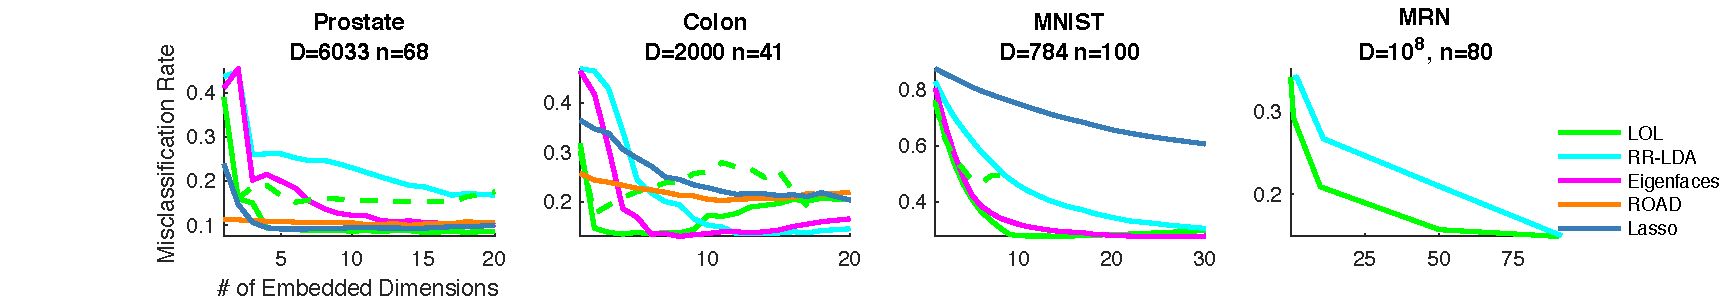
\includegraphics[width=1.0\textwidth]{../../figs/plot_real}
    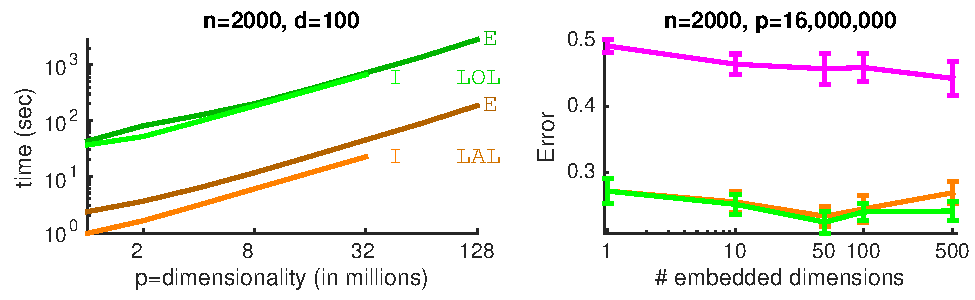
\includegraphics[width=0.7\textwidth]{../../figs/scalability}
    \caption{Top: LOL outperforms essentially all other methods for essentially all problems and number of dimensions to embed into.  Bottom: LOL (green) and LAL (brown, using random projections to approximate) for both fully in memory (IE) and semi-external memory (E) implementations.  Magenta compares performance to our scalable implementation of eigenfaces on the same problem.   }
		\label{fig:lolall}
		\end{cframed}
\end{figure}


\clearpage
\end{document}
